
\section{Computational Models}

While only Serpent 2.0 \cite{leppanenjaakko_serpent_2015} is used in this thesis, work to improve HTGR modeling in one program can inform efforts in another.  Therefore, modeling software beyond Serpent 2.0 is discussed in this chapter.

\subsection{Serpent}

In order to create and model complex geometries, Serpent uses constructive solid geometry (CSG), which defines homogeneous material cells using user-defined universes, cells, lattices, and specially-defined nested objects to define particle and pebble geometries.  Using these special objects and the particle dispersal routine in Serpent, TRISO particles and pebble bed reactors can be modeled.  Serpent has been tested with up to 60 million individual particles \cite{noauthor_serpent_nodate}.

Physics are based on a combination of classical kinematics, ENDF reaction laws, and random sampling.  For particle transport, Serpent uses surface tracking and Woodcock-delta tracking.  For material data, Serpent uses ACE format libraries for microscopic cross sections, and pre-generates macroscopic cross sections before beginning transport.  To further speed-up calculations, Serpent uses a unionized energy grid.  Serpent has been validated against MCNP, and validation is ongoing for radiation shielding and criticality safety analysis.  While the differences between Serpent and other Monte Carlo codes are usually marginal, Serpent experiences the same issues validating its results as other Monte Carlo programs, related to small differences in data libraries \cite{noauthor_serpent_nodate}.

\subsection{Work in Other Software}

A 1996 effort to improve MCNP developed a new sampling method for Monte Carlo.  The version of MCNP that used the sampling model was dubbed MCNP-BALL.  After testing by performing isotopic inventory and criticality calculations , it was seen that the MCNP-BALL code could get results accurate to 0.2\%.  The work developing MCNP-BALL also answered a weakness in core modeling due related to difficulties in modeling reactors with a so-called "double-heterogeneity" - having two or more types of pebble in a single reactor \cite{murata_new_1997}.

An additional look into MCNP HTGR simulations examined the ability to model what would normally be a stochastic geometry with uniform modeling.  Specifically, TRISO particles and pebbles were placed in body centered tetragonal BCT and hexagonal close pack (HCP).  In general, it was found that for very low packing fractions, such as the values seen in TRISO-in-pebble packing, the particles are generally far enough away that the differences between two crystal lattice structures are insignificant.  In smaller cores with adequate reflectors, the differences between the pebble packing lattices were more significant, but manageable.  However, in unreflected cores and moderators that are not graphite, this is no longer true.  Additionally, the effect of completely homogenizing the coating of the TRISO particles - blending them with the graphite matrix - caused a noticeable change, specifically lowering $k_{eff}$.  For methods using less dramatic homogenization methods, such as blending the 4 TRISO coatings into one uniform layer, an appreciable decrease in computational load was observed, and the results were marginally different from the 4-coating model \cite{karriem_mcnp_2001}.

BEAU, or Burnup Equilibrium Analysis Utility \cite{cisneros_pebble_2013}, was developed to model depletion and multiple burnup states for a continuously refueled pebble bed reactor, using the multiple burnup state method (MBSM) to do so.  MBSM improves on most full-core pebble bed computational methods by modeling all burnup states for a pebble, rather than homogenizing them into a representative average pebble.

BEAU is a python-based coupling software that combines either MCNP5 or Serpent with ORIGEN2, using new interface inspired by the MOCUP code named mocup.py.  Mocup.py takes the output files from an MCNP5 or Serpent simulation, and compiles the information from the simulation into an object that can be used to run depletion simulations.  BEAU can be used for fuel cycle analysis and finding the maximum burnup equilibrium.  It has been bench-marked against results for a pebble-bed HTGR in INL's PEBBED and VSOP \cite{cisneros_pebble_2013}.

\subsection{Fuel Modeling}

BEAU was used to aid in the design of a pebble bed fluoride high temperature reactor, PB-FHR, named the Mark-1 PB-FHR \cite{cisneros_pebble_2013}.  Much of the analysis is beyond the scope of this thesis, however, the handling of pebble locations is of interest.  The Mark-1 PB-FHR handles pebble locations using a face-centered cubic (FCC) lattice in which all burnup states seen in the reactor are present.  If one assumes a uniformly mixed core, the closeness of the different burnup compositions in the lattice provide a fairly good estimation.

A more general study examined the effects of pebble packing on the core neutronics in an HTGR \cite{turkmen_effect_2012}.  Rather than model a full core, a unit cell was created as a reference.  The study considers body centered cubic (BCC) and hexagonal close-packed (HCP).  Instead of using a variety of compositions to represent an equilibrium, middle-of-life (MOL) core, an enrichment of 9.6\%  - lower than the standard ~15\% for fresh HTGR pebble-fuel - is assumed for all pebbles.  For each lattice configuration, the fuel/moderator (F/M) ratio was varied, and the effects on core neutronics and isotopic compositions examined.  No significant difference between BCC and HCP cells was found.  The study determined it would likely be impossible to select a truly 'optimal' energy spectrum vis-\`{a}-vis minimizing the accumulation of particularly harmful fission products.  The author concluded that F/M ratios less than 1/1 favor reducing actinide inventories, while ratios greater than 1/1 can reduce the generation of fission products that would corrode the layers of the TRISO fuel.

Earlier work on HTGRs by General Atomic determined the composition of discharged thorium/uranium prismatic fuel elements.  This study assumes fuel recycling to complement the breed/burn fuel cycle proposed.  Additionally, the fuel cycle assumes the reactor can start with an initial feed material of 93\% U-235, which is not currently feasible (at least in commercial reactors in the United States) \cite{hamilton_htgr_1976}.


\section{Modern HTGRs}

The following discusses more recent HTGR designs, which are the inspiration for Sangamon200 and Sangamon20.

\subsection{PBMR}

The PBMR is a South African pebble bed HTGR design.  While it did not ultimately make it to construction, its design has offered invaluable insight to later HTGR pebble bed designs.  The PBMR is largely based on the German High Temperature Reactor (HTR) designs, and has a nameplate thermal power of 400 MW, with inlet-outlet temperatures of 500 \textdegree C to 900 \textdegree C.  It is a modular design, with each unit containing a graphite moderated, helium-cooled core housed in a steel pressure vessel.  In accident scenarios, the PBMR would rely on passive safety features using conduction and convection to provide cooling.

\begin{figure}[h!]
\centering
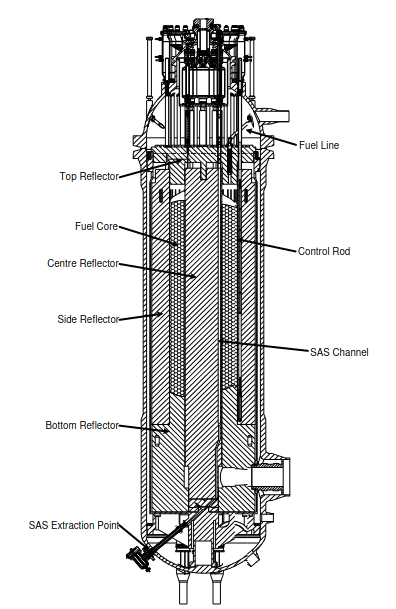
\includegraphics[width=0.5\linewidth]{figures/pbmr-v-cross-sect}
\caption{PBMR Schematic: Vertical Cross-section \cite{venter_pbmr_2005}}
\label{fig:pbmr-v-sect}
\end{figure}

Each core unit would hold around half a million pebbles, which used LEU based TRISO particles as the fuel form.  These TRISO particles are pressed into a 2.5cm radius graphite sphere, which then has an additional 0.5 cm thick layer of graphite pressed around it, to form a 3.0 cm radius pebble - around the size of a billiard ball.  The pebbles would undergo a six-pass multi-pass cycle to reach a target end burnup of 92,000 $\frac{MWd}{tU}$ \cite{venter_pbmr_2005}. 

\subsection{Next Generation Nuclear Plant (NGNP)}

Like the PBMR, the NGNP did not make it to construction.  However, the work in analyzing reactor designs and materials is still applicable to other work.  The NGNP project downselected its design choices to two models - a prismatic HTGR and a pebble-bed HTGR.  While the NGNP project eventually opted for the Areva prismatic HTGR design \cite{noauthor_areva_nodate} due to reasons related to pebble costs, it was noted that, technologically speaking, there was no inherent advantage or disadvantage bewteen the two technologies \cite{inl_basis_2011}.

Even though the reactor didn't make it to construction or operation, a plethora of research conducted in support of the NGNP project is applicable to similar reactors.  One such study is a whole-core depletion study of the the proposed prismatic HTGR design.

The reactor uses a once through fuel cycle, and assumed an average burnup of 100-150 $\frac{GWd}{t}$ after an 18 to 24 month stint in the core.  Much of the work from this study is applicable only to prismatic designs, namely the effects of the number of batches cycling, and fuel shuffling on core neutronics \cite{tkkim_whole-core_nodate}.

\subsection{X-energy}

Based on experience working on the PBMR project, the X-energy Xe-100 is a 200 MWt HTGR pebble-bed SMR.  It is similar in design to all of its predecessors, featuring LEU TRISO particle fuel in 3.0 cm radius pebbles.  While the Xe-100, or similar demonstration plant, has not been built as of this publication, the project is still ongoing.  It is this reactor, and by extension, the PBMR, that the micro-reactor described in this thesis is most heavily influenced by.

The Xe-100 uses approximately 220,000 pebbles in a six-pass cycle, and fuel pebbles identical to the ones intended for the PBMR \cite{harlan_x-energy_2018}.  However, while the number of passes is the same, the target end burnup for the pebbles is higher, at 160,000 $\frac{MWd}{tU}$ \cite{agnihotri_intrinsically_2017}.  Another key difference from the PBMR beyond size is the lack of central reflector.

While the Xe-100 has not been built, there have been studies conducted by ORNL providing data on the production and material properties of the PBMR-type fuel pebble.
